\chapter{INTRODUCTION}
\label{1.Chap:Intro}
% Refer Srinivas Bhaskar and Abroad theses for Chapter 1. \\\\
An electric power source that is directly connected to the distribution network or located at the meter's client site is known as distributed generation (DG) \cite{ACKERMANN2001195}. Main objectives of the DG are to provide a reliable and quality power to the end consumers. In the past two decades, the adoption of renewable energy sources (RESs) has been increasing to mitigate carbon emissions and build resilience to volatile energy prices from geopolitical wars. Also, the usage of power electronics based utility devices such as LED lighting systems, adjustable speed drives, etc., has been increased in the distribution system. The large penetration of RESs and power switching electronic devices (non-linear loads) into distribution system leads to power quality (PQ) degradation. The non-linear loads draw harmonic currents through the distribution network, resulting in voltage distortion and additional losses in the network. Further, these loads raise the demand for reactive power, which eventually causes the voltage variations such as sag and swell at the point of common coupling (PCC). All of these issues are the reasons for low power factor, inefficient distribution network, work interruption of sensitive equipment, and overheating of transformers and feeder lines \cite{ghosh2002power}. As a result, consumers and regulatory bodies that oversee and establish PQ standards became more aware of PQ issues. One of the widely accepted standards is IEEE-519 \cite{9848440}.  
 
 The installation of passive harmonic filters is the standard PQ improvement method used for many decades \cite{1268201}. The passive filters can improve the power factor of inductive loads and offer harmonic mitigation for DG systems. However, they may not be as effective as they could be due to a number of factors, including pre-tuned compensation frequencies, the formation of harmonic parallel and/or series resonances between the power system and the passive filter, and their component bulkiness \cite{1545766}. To overcome the problems with passive filters and to improve PQ in distribution system, active power filters (APFs) are developed \cite{4074559,1601573,gyugyi1976active,mohan1977active}. The APFs are referred as custom power devices (CPDs) when they are employed in distribution network. 
 
 \section{CUSTOM POWER DEVICES}
 
 Typically, the custom power devices (CPDs) are used to provide quality power to the end consumers in the distribution system. The CPDs can also be known as power quality conditioners (PQCs) as they provide quality power to the customers. The family of CPDs includes distribution static compensator (DSTATCOM), dynamic voltage restorer (DVR), unified power quality conditioner (UPQC), solid state transfer switch (SSTS), and solid state fault current limiter (SSFCL). In this section, a brief description of the DSTATCOM, DVR, and UPQC has been presented. 
 
 \subsection{Distribution Static Compensator} 
 
 The distribution static compensator (DSTATCOM), shunt connected custom power device, solves current-based quality problems in the distribution network. The DSTATCOM injects portion of load currents based on the requirement of consumer and/or distribution system operator (DSO) \cite{gyugyi1976active,nastran1994active,torrey1995single,hafner1997shunt}. For instance, to achieve unity power factor, harmonic filtering and load balancing at PCC, the DSTATCOM injects the load current components of harmonic, fundamental reactive, negative and zero sequence currents. The DSTATCOM is generally consists of a voltage source inverter (VSI), filter inductor and the DC storage capacitor as shown in Fig. \ref{fig1.1}.  



\begin{figure}[ht]
	\centering
		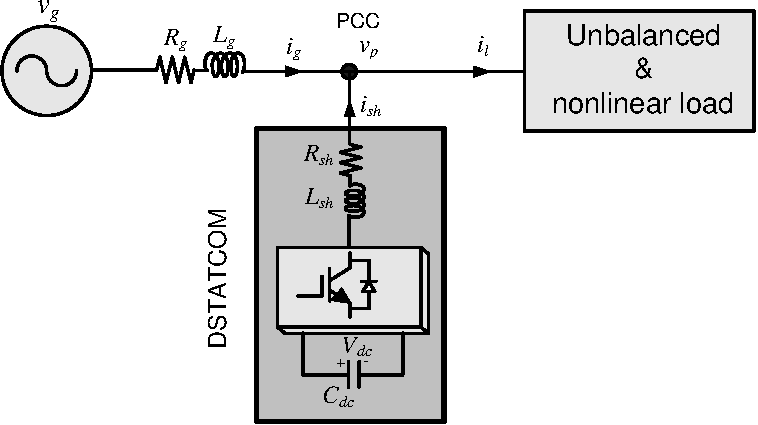
\includegraphics[scale=1]{figures/Chapter_1_2/fig1p1.pdf}	\caption{Single-line diagram of DSTATCOM}
	\label{fig1.1}
\end{figure}

 
 \subsection{Dynamic Voltage Restorer} 
 
 The dynamic voltage regulator (DVR), series connected custom power device, solves voltage-based quality problems in the distribution network. The DVR injects voltage in series with the grid voltage such that the load voltage is maintained as a balanced sinusoidal waveform with a desired amplitude \cite{moran1989line}. The primary goal of the DVR is to protect sensitive loads from voltage sag/swell, harmonics and interruptions in the supply side voltage  \cite{387140,woodley1999experience}. Fig. \ref{fig1.2} shows a single-line diagram of DVR system coupled to a distribution system. The DVR consists of VSI, LC filter, injection transformers and the DC storage capacitor.  
 
\begin{figure}[ht]
	\centering
		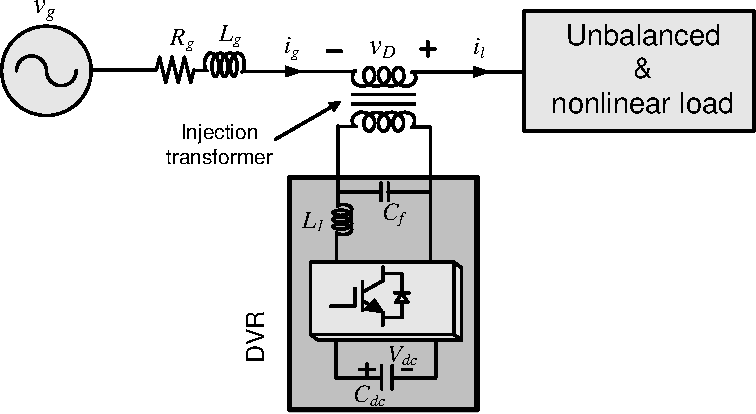
\includegraphics[scale=1]{figures/Chapter_1_2/fig1p2}
	\caption{Single-line diagram of DVR}
	\label{fig1.2}
\end{figure}

\vspace*{0.3cm}
\subsection{Unified Power Quality Conditioner}
 Unified power quality conditioner (UPQC) is relatively the latest device in the family of the custom power devices \cite{662847,chen2000unified,tolbert2000multilevel,mwinyiwiwa2000multiterminal,ghosh2001unified}.  The UPQC consists of both DSTATCOM and DVR with a common DC-link as shown in Fig. \ref{fig1.3}. Therefore, the UPQC can simultaneously fulfill the objectives of both DSTATCOM and DVR, i.e., solving both the current and voltage-based quality problems in the distribution network.


\begin{figure}[ht]
	\centering
		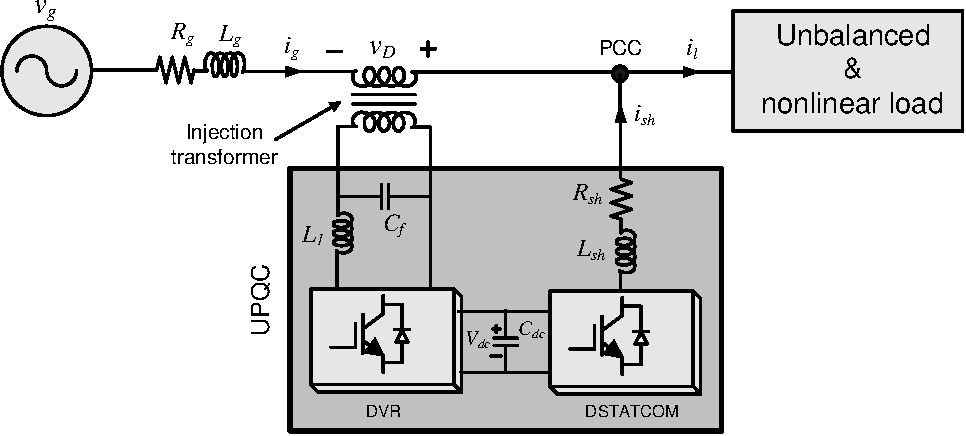
\includegraphics[scale=0.88]{figures/Chapter_1_2/fig1p3}
	\caption{Single-line diagram of UPQC}
	\label{fig1.3}
\end{figure}

Hybrid power filters, which include passive filters and active filters, are also discussed in the literature \cite{libano1997simplified,fujita2000hybrid,peng1993compensation}. These hybrid filters incorporate the advantages of both active and passive filters. Additionally, the passive filters help in decreasing the active filter's rating.

The present work focuses on the use of DSTATCOM and DVR individually in the power distribution network. The problems identified in these areas serve as a motivation for the use of UPQC system as it is a combination of DSTATCOM and DVR. The motivations of this work are described in the following section.

\section{MOTIVATION}

 The unified power quality conditioner (UPQC) with back-to-back (BTB) configuration is a flexible custom power device that can improve system performance against both current and voltage related PQ issues. The realization of UPQC, in general any power electronics inverter based system, involves three essential aspects. The first one is the selection of the suitable VSI topology. The second one is the selection of suitable algorithms for generation of reference quantities. The third one is the selection of the suitable controller to realize VSI currents and/or voltages track their respective reference quantities. 
 
 The main requirements before selecting the VSI topology can be listed as:
 \begin{itemize}
 \item The DC-link voltage rating is selected such that it has no impact on the ability of power conversion unit to deliver the satisfactory performance. 
 \item The power conversion unit must be compact, efficient and high power density. These features can be achieved by using the power conversion unit with least number of power semiconductor switches and/or with wide-band semiconductor switches. 
 \item The VSI topology must be able to provide path for the flow of zero sequence currents and inject zero sequence voltages into the distribution network.
 \end{itemize}
 The series converter of the BTB configured UPQC is almost idle most of the time, since the occurrence of voltage related issues is less often. Thus, the converter utilization is poor with BTB configuration. To improve the converter utilization factor without affecting UPQC's ability to generate required voltages and currents, the reduced switch count converter topologies can be considered.
 
 Various algorithms for generation of reference currents are reported in the literature for DSTATCOM, such as instantaneous reactive power theory \cite{akagi1984instantaneous, akagi1986control}, generalized instantaneous reactive power theory \cite{akagi1983generalized,peng1996generalized}, Synchronous reference frame theory \cite{1629027}, theory of instantaneous symmetrical components \cite {ghosh2000use} etc. Similarly, various algorithms for generation of reference voltages are reported in the literature for DVR, such as pre-sag, in-phase, energy-optimized compensations, dual instantaneous active-reactive power theory \cite{6556997, 1208380, 1510825, 8400555} etc. The generation of these reference quantities requires approaches for accurate extraction of fundamental frequency positive sequence (FFPS) components and phase angle of grid voltages. Therefore, the extraction of FFPS components based on the operators: second order generalized integrator (SOGI), cascaded delayed signal cancellation (CDSC) and multiple delayed signal cancellation (MDSC) are to be explored and selected the operator with superior characteristics for the UPQC operation.    
 
 There are various switching control strategies or controllers to realize the currents and/or voltages of the power conversion unit. 
 Some of these controllers reported in literature are proportional-intergral (PI) and/or proportional-resonant (PR) controller(s) \cite{8170301,8345740,4305325,1629027, 5398914, 6880399}, hysteresis controller \cite{4158027,malesani1990novel,8846889}, model predictive controller \cite{6939709,9175195}, sliding mode controller \cite{9108551,8264745,6563653,7776961,9264672,8466115,7506128} etc. The main requirements before selecting the controller can be listed as:
 \begin{itemize}
 \item Control instantaneous currents and/or voltages without amplitude and phase errors.
 \item Provide high dynamic performance of the power conversion unit.
 \item Provide limited and constant switching frequency operation to protect the power semiconductor switches and increase the efficiency of the power conversion unit.
 \item Robust to variations in load and network parameters. 
 \item Simple to implement and low cost.
 \item The total harmonic distortion (THD) levels should be within the limits specified in the standards.
 \end{itemize}
 Considering the above requirements, specifically the insensitive to the model parameter variations, the sliding mode controller is considered for the UPQC system. The sliding mode control scheme can be implemented in any one of the reference frames: $dq$, $\alpha \beta$ and natural reference frame ($abc$). Due to availability of generation of reference voltages/currents in $abc$ frame, implementing a controller in the same reference frame would reduce the computational burden and the signal transformation errors. However, the three-phase three-leg or four-leg voltage source converters suffer from the coupling issue in $abc$ frame. The dynamics of each state variable depends on the control inputs of all the legs of the converter. This coupling leads to difficulty in assigning appropriate values to the control inputs using a conventional sliding surface in sliding mode control (SMC) scheme. Therefore, it is necessary to propose a new sliding surface which can provide a per-phase analysis of the system irrespective of the inherent coupling nature in the $abc$ frame. 
 
 \section{OBJECTIVES}

The most widely used converter configuration for the UPQC is back-to-back (BTB) converter \cite{6095377, iet-pel.2010.0134, 5688329,5393074, ghosh2001unified, 5235743,5672403, 4483694}. The BTB configuration contains two VSIs with 16 semiconductor switches in three-phase four-wire (3P4W) distribution system. As described in the previous section, to increase the converter utilization factor, recently proposed dual-output converter (DOC) can be considered for UPQC system \cite{4348103}. The DOC used in three-phase three-wire (3P3W) distribution system can be called as nine-switch converter (NSC) as it contains only 9 semiconductor switches \cite{5713844}.  The DOC used in 3P4W DG system can be called as twelve-switch converter (TSC) as it contains 12 switches. For both 3P3W and 3P4W DG systems, the required switches in DOC is 25\% less than the switches in BTB configuration. The UPQC was designed using NSC for 3P3W DG system in \cite{5713844,7018088} and using TSC for 3P4W DG system in \cite{6301686}. Nevertheless, the compensation capabilities of UPQC with DOC have been analyzed only with linear controllers in $dq$ frame. Alternative control techniques can be applied to improve the performance of DOC based UPQC system.    

This thesis is focused to develop a new sliding mode control scheme for each four-leg VSI based DSTATCOM and DVR in the natural $abc$ frame. Finally, the developed control scheme is applied to the DOC based UPQC. Based on the literature survey and the motivations, the objectives of the thesis are formulated as given below:

\begin{enumerate}
\begin{spacing}{1.5}
\item To explore and investigate the advanced approaches to extract an accurate FFPS components and phase angle of grid voltages. This is essential for the improved compensation ability of all custom power devices in the DG system.

\item{To demonstrate the problems associated with the conventional sliding mode control scheme while developing for four-leg VSI based systems in the natural reference frame.} 

\item To propose an improved sliding mode control scheme which would provide the control design flexibility in the natural reference frame, incorporate the control of converter neutral-point voltage in addition to control of converter currents and/or voltages and incorporate desired robustness to the parametric variations and uncertainties in the system. 

\item{Validation of proposed control scheme on four-leg VSI based DSTATCOM and DVR, and DOC based UPQC through simulation and experimental studies.}
\end{spacing}
\end{enumerate}


\section{ORGANIZATION OF  THE THESIS}

The reasons for the degradation of power quality, its effects and the PQ standard in the DG system are presented in \textbf{Chapter \ref{1.Chap:Intro}}. To address the PQ issues in the DG system, various solutions such as passive filters, active filters or custom power devices and hybrid filters are described. Various custom power devices are briefly discussed as they are flexible solution for PQ improvement in DG system. Finally, motivations and objectives of the thesis are presented.


\textbf{Chapter \ref{2.Chap:DOCIntro}} provides an introduction to the conventional or back-to-back UPQC connected to the 3P3W distributed generation (DG) system. It offers a brief overview of the recently proposed nine-switch converter and highlights its advantages and drawbacks compared to the back-to-back topology. The chapter also presents the previously designed nine-switch UPQC, including its control methods and associated challenges. Furthermore, the chapter delves into the discussion of control techniques that are being considered as replacements for the current linear control methods used in the nine-switch UPQC. These alternative control techniques are explored in order to overcome the limitations of the existing linear control methods.

\textbf{Chapter \ref{3.Chap:PLL}} presents different operators, such as the second-order generalized integrator (SOGI), cascaded delayed signal cancellation (CDSC), and multiple delayed signal cancellation (MDSC). These operators are utilized to extract the fundamental positive sequence components from signals that are distorted and unbalanced. Independently, these operators are cascaded to the synchronous reference frame phase-locked loop (SRF-PLL) to precisely determine the phase angle of the grid voltages. Through simulation studies, the performance of PLLs employing these three operators is thoroughly analyzed. 


\textbf{Chapter \ref{4.Chap:DSTATCOM}} introduces a novel sliding mode control (SMC) approach for the four-leg distribution static compensator (DSTATCOM). The proposed control scheme utilizes a new sliding surface, allowing for simultaneous control of both compensator currents and the converter neutral-point voltage (NPV). The inclusion of NPV control is crucial for power quality conditioners based on dual-output converters. To assess the effectiveness of the proposed control scheme, extensive simulation and experimental studies are conducted on the four-leg DSTATCOM system.

In \textbf{Chapter \ref{5.Chap:DVR}}, a new sliding mode control (SMC) approach is introduced for the four-leg dynamic voltage restorer (DVR). The proposed control scheme incorporates a novel sliding surface, enabling concurrent control of compensator voltages and the converter neutral-point voltage (NPV). This inclusion of NPV control is particularly significant for power quality conditioners utilizing dual-output converters. To evaluate the effectiveness of the proposed control scheme, comprehensive simulation and experimental studies are carried out on the four-leg DVR system.

\textbf {Chapter \ref{6.Chap:DOCUPQC}} addresses the extension of the control schemes proposed in Chapter \ref{4.Chap:DSTATCOM} for DSTATCOM and Chapter \ref{5.Chap:DVR} for DVR to dual-output converter (DOC) based unified power quality conditioner (UPQC) applications. The proposed control scheme allows for the simultaneous control of both converter NPVs and compensator voltages and currents. By incorporating NPV control into the controller, the proposed scheme can be implemented directly in the natural frame. A comprehensive model of the proposed control scheme is developed for the DOC-based left shunt UPQC (UPQC-L) system. A novel reference generation approach has also been proposed for the
neutral-point voltages in the UPQC-L application. To validate the effectiveness of the proposed scheme, extensive simulation studies are conducted on the DOC-based UPQC-L system. 

In \textbf {Chapter \ref{7.Chap:Conclusions}}, important conclusions derived from the research work are presented. These conclusions encapsulate the key findings and outcomes of the study. Additionally, suggestions for future directions and potential areas for further research are outlined, providing a roadmap for future work in the field. Furthermore, the \textbf {Appendix A} %contains detailed information about the experimental setup, including accompanying photographs. This supplementary material offers a visual representation of the setup and enhances the understanding of the experimental procedures and equipment utilized in the study.
provides a simplified explanation of the control schemes proposed for both DSTATCOM and DVR systems, while \textbf{Appendix B} outlines the motivation behind utilizing a four-leg converter for DVR application due to the limitations of three-wire DVR in distribution systems.